\documentclass{article}
\usepackage[utf8]{inputenc}
\usepackage[english]{babel}
\usepackage{amsmath}
\usepackage[]{amsthm}
\usepackage[]{amssymb} 
\usepackage{mathrsfs}
\usepackage{tcolorbox}
\usepackage{nicefrac}
\usepackage{mathtools}
% \usepackage{graphicx}
\usepackage{caption}
\usepackage{subcaption}
\usepackage{array}

\graphicspath{ {./images/} }

\theoremstyle{definition}
\newtheorem*{claim}{Claim}
\newtheorem*{corollary}{Corollary}
\DeclareMathOperator{\adj}{\operatorname{adj}}
\DeclareMathOperator{\im}{\operatorname{im}}
\DeclareMathOperator{\spn}{\operatorname{span}}
\DeclareMathOperator{\nll}{\operatorname{null}}
\newcommand{\trace}{\operatorname{trace}}
\newcommand{\R}{\mathbb{R}}
\newcommand{\Z}{\mathbb{Z}}
\newcommand{\N}{\mathbb{N}}
\newcommand{\F}{\mathbb{F}}
\newcommand{\C}{\mathbb{C}}
\newcommand{\D}{\operatorname{D}}
\newcommand{\GL}{\operatorname{GL}}
\newcommand{\SL}{\operatorname{SL}}
\newcommand{\GLnR}{\GL_n(\R)}
\newcommand{\SLnR}{\SL_n(\R)}
\DeclarePairedDelimiter\floor{\lfloor}{\rfloor}
\DeclarePairedDelimiter\set{\{}{\}}
\DeclarePairedDelimiter\abs{\lvert}{\rvert}
\DeclarePairedDelimiter\genby{\langle}{\rangle}
\DeclarePairedDelimiter\bilform{\langle}{\rangle}
\newcommand{\restrict}[1]{ \big|_{#1} }
\newcommand{\evalat}[2]{\Big|_{#1}^{#2}}


\title{18.701: Problem Set 10}
\author{Dmitry Kaysin}
\date{August 2020}
\begin{document}
\maketitle 


\subsection*{Problem 1}

\begin{tcolorbox}
a) Let $\SL_2$ be the special linear group of real matrices with determinant $1$.
Determine the possible eigenvalues $\lambda$ (real or complex) of the elements of $\SL_2$, and make a drawing showing the points $\lambda$ in the complex plane.
\end{tcolorbox}

We start with $2 \times 2$ matrix of the form
\[
    A =
    \begin{pmatrix}
        a & b \\
        c & d
    \end{pmatrix}
\]
with $\det A = ad - bc = 1$.

Characteristic polynomial of $A$ is $t^2 - tr + 1$ where $r = \trace A = a+d$.
Eigenvalues of $A$ are thus
\[
    \lambda = \frac{r \pm \sqrt{r^2-4}}{2}.
\]
As $r \to \infty : \lambda \to \pm \infty$ and
as $r \to -\infty : \lambda \to \mp 0$.
For $r$ in the interval $(-\infty, -2] \cup [2, \infty)$ eigenvalues of $A$ are real.
For $r$ in the interval $(-2, 2)$ eigenvalues of $A$ are complex, occur in conjugate pairs and their locus is upper and lower half of the unit circle on the complex plane.

\begin{figure}[h]
    \caption{Possible eigenvalues of $A \in \SL_2$ in the complex plane.}
    \centering
    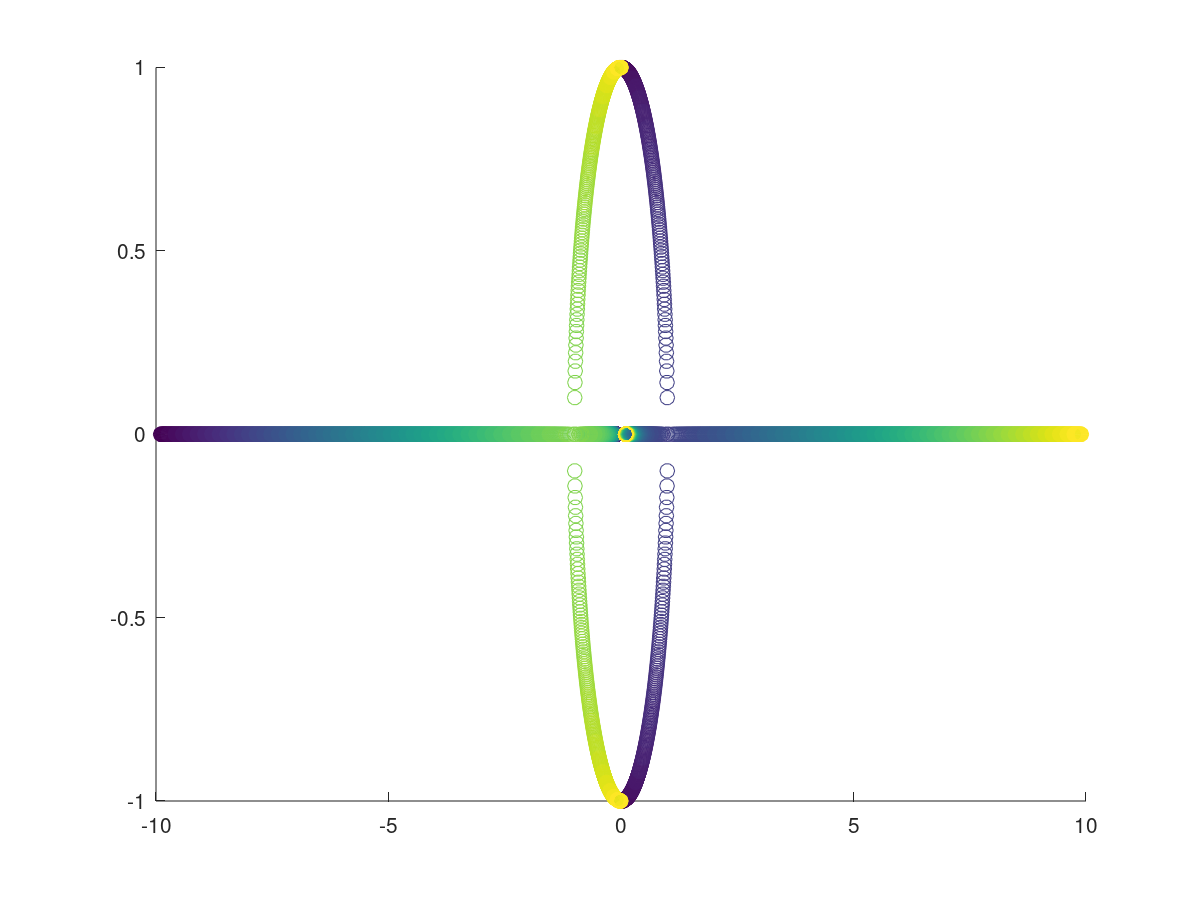
\includegraphics[width=0.8\textwidth]{ps10p1}
\end{figure}


\begin{tcolorbox}
b) For each $\lambda$, decompose the set of matrices $P \in \SL_2$ with eigenvalue $\lambda$ into $\SL_2$-conjugacy classes.
\end{tcolorbox}

\begin{proof}

We claim that for every matrix $A$ with complex eigenvalues $\lambda$ and $\overline{\lambda}$ there exists a matrix $Q \in \SL_2$ such that 
$Q^t A Q = \Lambda = \begin{pmatrix} \lambda & \\ & \overline{\lambda} \end{pmatrix}$.

Let $X = (u, v)^t$ be a unit eigenvector of $A$ with eigenvalue $\lambda$.
Then $Y = (-v,u)^t$ is also a unit eigenvector of $A$ with eigenvalues $\overline{\lambda}$. [PROVE]
Let 
$
    Q =
    \begin{pmatrix}
        u & -v \\
        v & u
    \end{pmatrix}
$, then
\begin{align*}
    Q^t A Q & = 
    \begin{pmatrix}
        u & v \\
        -v & u
    \end{pmatrix}
    \begin{pmatrix}
        a & b \\
        c & d
    \end{pmatrix}
    \begin{pmatrix}
        u & -v \\
        v & u
    \end{pmatrix}
    =
    \begin{pmatrix}
        u & v \\
        -v & u
    \end{pmatrix}
    \begin{pmatrix}
        \lambda u & -\overline{\lambda} v \\
        \lambda v & \overline{\lambda} u
    \end{pmatrix}
    \\
    & = 
    \begin{pmatrix}
        \lambda(u^2+v^2) & - \overline{\lambda} uv + \overline{\lambda} uv \\
        - \lambda uv + \lambda uv & \overline{\lambda} (v^2 + u^2)
    \end{pmatrix}
    = 
    \begin{pmatrix}
        \lambda &  \\
         & \overline{\lambda}
    \end{pmatrix}.
\end{align*}


\end{proof}

\begin{tcolorbox}
c) Determine the matrices $P \in \SL_2$ that can be obtained as $P = e^A$ for some real matrix $A$.
\end{tcolorbox}

\begin{proof}
\end{proof}

\subsection*{Problem 2}

\begin{tcolorbox}
According to Sylvester's Law, every $2 \times 2$ real symmetric matrix is congruent to exactly one of six standard types.
List them.
If we consider the operation of $\GL_2$ on $2 \times 2$ matrices by $P * A = PAP^t$, then Sylvester's Law asserts that the symmetric matrices form six orbits.
We may view the symmetric matrices as points in $\R^3$, letting $(x,y,z)$ correspond to the matrix
$
\begin{pmatrix}
    x & y \\
    y & z
\end{pmatrix}
$.
Describe the decomposition of $\R^3$ into orbits geometrically, and make a clear drawing depicting it.
\end{tcolorbox}

According to the Sylvester's Law, every symmetric $2 \times 2$ matrix is congruent to one of the following six "signature" matrices (unique up to permutation of basis vectors / diagonal entries):
\begin{gather*}
	I_{(2,0,0)} = 
	\begin{pmatrix}
		1 &  \\
		 & 1
	\end{pmatrix},
	\quad
	I_{(1,0,1)} = 
	\begin{pmatrix}
		1 &  \\
		 & 0
	\end{pmatrix}
	\sim
	\begin{pmatrix}
		0 &  \\
		 & 1
	\end{pmatrix},
	\\
	I_{(0,2,0)} =
	\begin{pmatrix}
		-1 &  \\
		 & -1
	\end{pmatrix},
	\quad
	I_{(0,1,1)} = 
	\begin{pmatrix}
		-1 &  \\
		 & 0
	\end{pmatrix}
	\sim
	\begin{pmatrix}
		0 &  \\
		 & -1
	\end{pmatrix},
	\\
	I_{(0,0,2)} =
	\begin{pmatrix}
		0 & 0 \\
		0 & 0
	\end{pmatrix},
	\quad
	I_{(1,1,0)} =
	\begin{pmatrix}
		1 &  \\
		 & -1
	\end{pmatrix}
	\sim
	\begin{pmatrix}
		-1 &  \\
		 & 1
	\end{pmatrix}.
\end{gather*}

We also note that since $\GL_2$ is connected, orbit of each "signature" matrix must also be connected.
Since no pair of "signature" matrices is connected, orbits of "signature" matrices are disjoint.
Moreover, orbits of the "signature" matrices partition the space of $2 \times 2$ matrices and $\R^3$.

We now examine orbits in $\R^3$ of six "signature" matrices.
Consider arbitrary matrix $P$ in $\GL_2$ with $\det P \neq 0$:
\[
	\begin{pmatrix}
		a & b \\
		c & d
	\end{pmatrix},
	\quad ad-bc \neq 0.
\]

\paragraph{Case 1: $I_{(2,0,0)}$}

\begin{align*}
	P * I_{(2,0,0)} & =
	P I_{(2,0,0)} P^t =
	\begin{pmatrix}
		a & b \\
		c & d
	\end{pmatrix}
	\begin{pmatrix}
		1 & 0 \\
		0 & 1
	\end{pmatrix}
	\begin{pmatrix}
		a & c \\
		b & d
	\end{pmatrix}
	=
	\begin{pmatrix}
		a^2+b^2 & ac+bd \\
		ac+bd & a^2+b^2
	\end{pmatrix}
	\\
	& = (a^2+b^2, ac+bd, a^2+b^2)
	= (v_1 \cdot v_1, v_1 \cdot v_2, v_2 \cdot v_2)
	\\
	& = (\abs{v_1}^2, \abs{v_1}\abs{v_2}\cos\phi, \abs{v_1}^2),
\end{align*}
where $v_1 = (a,b)^t$, $v_2 = (c,d)^t$ and $\phi$ is an oriented angle between $v_1$ and $v_2$.
We note that $v_1$ and $v_2$ must be nonzero and must not be collinear, otherwise determinant of $P$ would be equal to $0$; therefore $v_1 \neq 0, v_2 \neq 0$ and $\phi \in (0,\pi) \cup (\pi, 2\pi)$.

Since $\abs{v_1}$ and $\abs{v_2}$ can be any positive real number, the orbit of $I_{(2,0,0)}$ under conjugation by an element of $\GL_2$ is a subset of $\R^3$
\[
	\GL_2 (I_{(2,0,0)}) = \set{(r^2, \lambda rs, s^2): r,s \in (0, \infty), \lambda \in (-1,1)}.
\]
By inspection, the orbit is an interior of a positive cone. 

\paragraph{Case 2: $I_{(1,0,1)}$}

\begin{align*}
	P * I_{(1,0,1)} & =
	P I_{(1,0,1)} P^t =
	\begin{pmatrix}
		a & b \\
		c & d
	\end{pmatrix}
	\begin{pmatrix}
		1 & 0 \\
		0 & 0
	\end{pmatrix}
	\begin{pmatrix}
		a & c \\
		b & d
	\end{pmatrix}
	=
	\begin{pmatrix}
		a^2 & ac \\
		ac & c^2
	\end{pmatrix}
	\\
	& = (a^2, ac, c^2).
\end{align*}

Therefore the orbit of $I_{(1,1,0)}$ under conjugation by an element of $\GL_2$ is a subset of $\R^3$
\[
	\GL_2 (I_{(1,1,0)}) = \set{(a^2, ac, c^2): a,c \in \R^\times}.
\]
By inspection, the orbit is a positive cone with the vertex removed. 

\begin{figure}[h]
    \caption{Cones that are the orbits of $I_{(1,0,1)}$ and $I_{(0,1,1)}$. Orbits of $I_{(2,0,0)}$ and $I_{(0,2,0)}$ are interior of these cones. Zero point is removed.}
    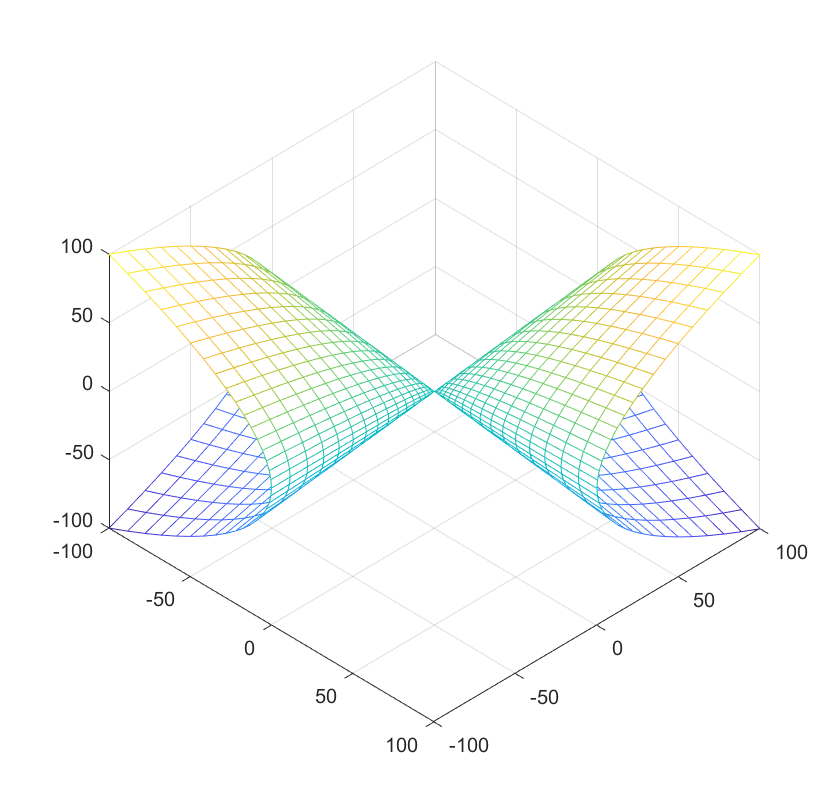
\includegraphics[width=0.8 \textwidth]{Both.png}
    % \begin{subfigure}{0.5\textwidth}
    %     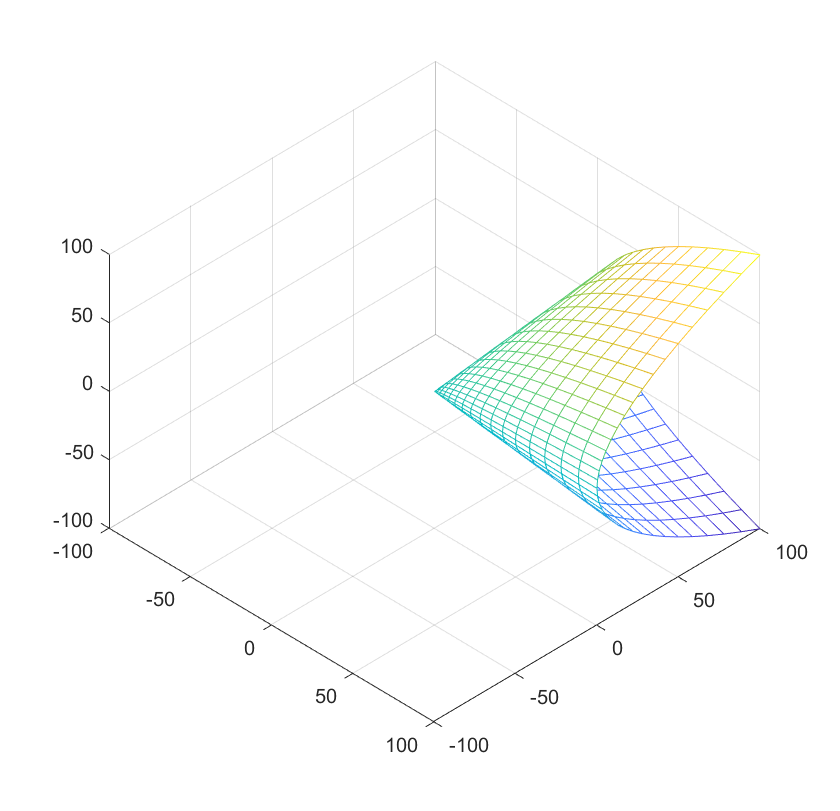
\includegraphics[width=\linewidth]{(1,0,1).png}
    % \end{subfigure}
    % \begin{subfigure}{0.5\textwidth}
    %     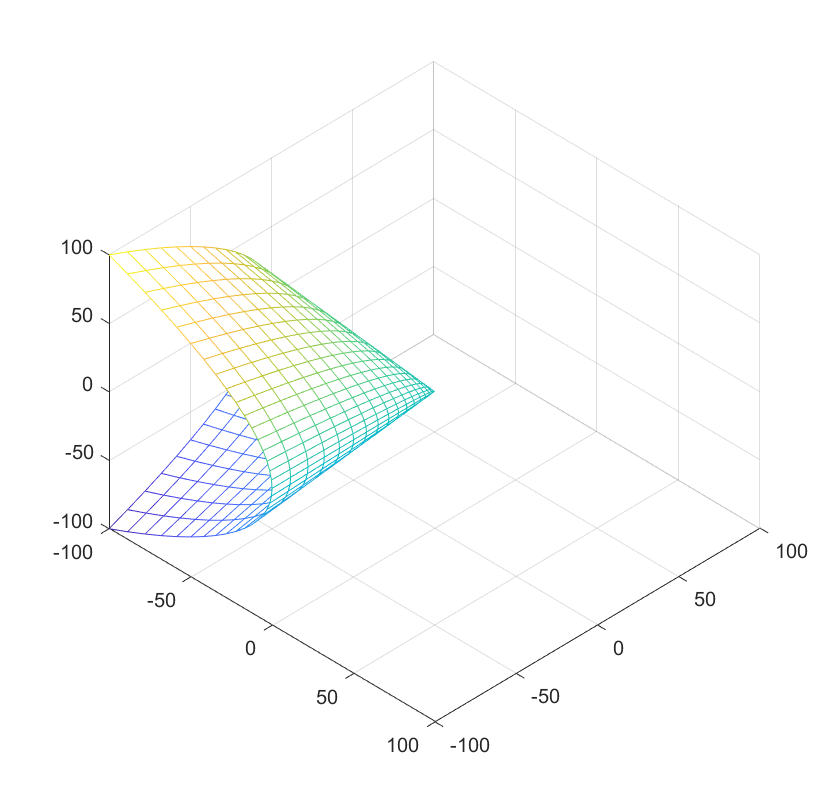
\includegraphics[width=\linewidth]{(0,1,1).png}
    % \end{subfigure}
\end{figure}

\paragraph{Case 3: $I_{(0,2,0)}$}

\[
	P * I_{(0,2,0)} = P I_{(0,2,0)} P^t = - P I_{(2,0,0)} P^t.
\]
From this we can see that the orbit of $I_{(0,2,0)}$ under conjugation is
\[
	\set{(-r^2, \lambda rs, -s^2) \> : \> r,s \in (0, \infty), \lambda \in (-1,1)},
\]
which is an interior of a negative cone. 

\paragraph{Case 4: $I_{(0,1,1)}$}

\[
    P * I_{(,1,1)} = P I_{(0,1,1)} P^t = - P I_{(1,0,1)} P^t.
\]
Therefore the orbit of $I_{(0,1,1)}$ under conjugation is
\[
	\GL_2 (I_{(0,1,1)}) = \set{(-a^2, ac, -c^2): a,c \in \R^\times},
\]
which is a negative cone with the vertex removed. 

\paragraph{Case 5: $I_{(0,0,2)}$}

\[
	P * I_{(0,0,2)} = P I_{(0,0,2)} P^t = I_{(0,0,2)}.
\]
The orbit of $I_{(0,0,2)}$ under conjugation is $I_{(0,0,2)} = (0,0,0)$.

\paragraph{Case 6: $I_{(1,1,0)}$}

Since orbits of "signature" matrices partition $\R^3$, the only remaining subset of $\R^3$ is the exterior of a double cone.

Curiously, the orbit of $I_{(1,1,0)}$ can be parameterized via a function $\varphi : \C \times \C \to \R^3$:
\begin{equation} \label{eq:case6}
    \varphi(z_1, z_2) =
    \begin{pmatrix}
        \Re (z_1^2) \\
        \Re (z_1 z_2) \\
        \Re (z_2^2)
    \end{pmatrix}
\end{equation}

\begin{proof}

\begin{align*}
	P * I_{(1,1,0)} & =
	P I_{(1,1,0)} P^t =
	\begin{pmatrix}
		a & b \\
		c & d
	\end{pmatrix}
	\begin{pmatrix}
		1 & 0 \\
		0 & -1
	\end{pmatrix}
	\begin{pmatrix}
		a & c \\
		b & d
	\end{pmatrix}
	=
	\begin{pmatrix}
		a & b \\
		c & d
	\end{pmatrix}
	\begin{pmatrix}
		a & c \\
		-b & -d
	\end{pmatrix}
	\\
	& =
	\begin{pmatrix}
		a^2-b^2 & ac-bd \\
		ac-bd & c^2-d^2
	\end{pmatrix}
	=
	\begin{pmatrix}
    	a^2-b^2 \\
    	ac-bd \\
    	c^2-d^2
	\end{pmatrix},
\end{align*}
which produces an expression equivalent to (\ref{eq:case6}) for complex numbers $z_1 = a+bi, z_2 = c+di$.

\end{proof}


\subsection*{Problem 3}

\begin{tcolorbox}
This problem is about the space $V$ of real polynomials in the variables $x$ and $y$.
If $f$ is a polynomial, $\partial_f$ will denote the operator 
$f \left( \frac{\partial}{\partial x}, \frac{\partial}{\partial y} \right)$,
and $\partial_f(g)$ will denote the result of applying this operator to a polynomial $g$.

a) The rule $\bilform{f,g} = \partial_f(g)_0$ defines a bilinear form on $V$, the subscript denoting evaluation of a polynomial at the origin.
Prove that this form is symmetric and positive definite, and that the monomials $x^i y^j$ form an orthogonal basis of $V$.
\end{tcolorbox}

\begin{proof}

Let $f = x^i y^j, g = x^k y^n$.

If $j > n$ then
\[
	\bilform{f,g} 
	= D_x^i D_y^j x^k y^n 
	= n! \> D_x^i D_y^{j-n} x^k
	= 0.
\]
Similarly, if $i > k$, we have $\bilform{f,g} = 0$.

If $j < n$ while $i \leq k$ then
\[
	\bilform{f,g} 
	= D_x^i D_y^j x^k y^n 
	= n (n-1) \cdots (n-j+1) \cdot k (k-1) \cdots (k-i+1) \cdot x^{k-i} y^{n-j},
\]
which evaluates to $0$ at the origin.
Similarly, if $i < k$ while $j \leq n$ , we have $\bilform{f,g} = 0$.

Finally, if $i = k, j = n$, we have
\[
	\bilform{f,g}
	= D_x^i D_y^j x^i y^j
	= (i!) (j!)
\]
It is now easy to see that $\bilform{f,g} = \bilform{g,f}$ for any monomials $f$ and $g$.
Since monomials form a basis of $V$, this result carries over to an arbitrary polynomial.
This proves that $\bilform{\cdot,\cdot}$ is symmetric, as required.

Moreover, as we have seen previously, monomials $f = x^i y^j$ and $g = x^k y^n$ are orthogonal with respect to $\bilform{\cdot,\cdot}$ unless $i = k, j = n$.
This proves that the basis of monomials is orthogonal, as required.

For nonzero $f = \sum_i \sum_j a_{ij} \> x^i y^j$ we have:
\[
	\bilform{f,f}
	= \sum_i (i!)^2,
\]
which is always positive since $i > 0$.
We conclude that $\bilform{\cdot,\cdot}$ is positive definite, as required.

\end{proof}


\begin{tcolorbox}
b) We also have the operator of multiplication by $q$, which we write as $m_q$.
So $m_q(g) = qg$.
Prove that $\partial_q$ and $m_q$ are adjoint operators.
\end{tcolorbox}

\begin{proof}

Operators $\partial_q$ and $m_q$ are adjoint if
\begin{equation} \label{eq:adjoint}
    \bilform{\partial_q f, g} = \bilform{f, m_q g} \text{ for all $f, g$}.
\end{equation}

Consider monomials $f = x^i y^j, g = x^k y^n$ and $q = x^r y^s$.

\[
    \partial_q (f)
    = D_x^r D_y^s x^i y^j
    = \frac{i!}{(i-r)!} \frac{j!}{(j-s)!} x^{i-r} y^{j-s},
\]
\[
    \bilform{\partial_q (f), g} 
    = \frac{i!}{(i-r)!} \frac{j!}{(j-s)!} \bilform{x^{i-r} y^{j-s}, x^k y^n}
\]

\paragraph{Case 1: $i-r = k$ and $j-s = n$.}
Evaluating the left-hand side of (\ref{eq:adjoint}) we have:
\[
    \bilform{\partial_q (f), g} 
    = \frac{i!}{k!} \frac{j!}{n!} \bilform{x^k y^n, x^k y^n}
    = \frac{i!}{k!} \frac{j!}{n!} \> k! \> n! 
    = (i!) (j!).
\]
Evaluating the right-hand side of (\ref{eq:adjoint}) we have:
\[
    \bilform{f, m_q(g)} 
    = \bilform{x^i y^j, x^{k+r} y^{n+s}}
    = \bilform{x^i y^j, x^i y^j}
    = (i!) (j!).
\]
Therefore, $\bilform{\partial_q (f), g} = \bilform{f, m_q(g)}$

\paragraph{Case 2: $i-r \neq k$ or $j-s \neq n$.}
Evaluating the left-hand side of (\ref{eq:adjoint}) we have:
\[
    \bilform{\partial_q (f), g} 
    = \frac{i!}{(i-r)!} \frac{j!}{(j-s)!} \bilform{x^{i-r} y^{j-s}, x^k y^n}
    = 0.
\]
Evaluating the right-hand side of (\ref{eq:adjoint}) we have:
\[
    \bilform{f, m_q(g)} 
    = \bilform{x^i y^j, x^{k+r} y^{n+s}}
    = 0.
\]
We conclude that $\partial_q$ and $m_q$ are adjoint operators.

\end{proof}


\begin{tcolorbox}
c) When $f = x^2 + y^2$, the operator $\partial_f$ is the Laplacian, which is often written as $\Delta$.
A polynomial $h$ is harmonic if $\Delta h = 0$.
Let $H$ denote the space of harmonic polynomials.
Identify the space $H^\perp$ orthogonal to $H$ with respect to the given form.
\end{tcolorbox}

Consider arbitrary $h \in H$ and $g \in V$.
Since $\partial_f$ and $m_f$ are adjoint operators, we have:
\begin{gather*}
	\bilform{\partial_f(h), g} = \bilform{h, m_f(g)}, \\
	\intertext{by definition of $H$ we have $\partial_f(h) = 0$, thus:}
	\bilform{0, g} = \bilform{h, fg}.
\end{gather*}
Since $\bilform{0, g} = 0$ for any $g$, we have $\bilform{h, fg} = 0$.
Therefore, $h$ and $fg$ are orthogonal.
Since $g$ can be arbitrary, harmonic polynomials are orthogonal to any polynomial divisible by $f = x^2+y^2$.
Denote $W$ the space of polynomials that are divisible by $f$.

To prove that any polynomial that is orthogonal to harmonic polynomials is in $W$, we need to show that $W \oplus H = V$.
We have already established that $H \cap W = 0$ since $H$ and $W$ are orthogonal, therefore it suffices to show that $H + W = V$, i.e. any polynomial $p \in V$ can be represented as a linear combination of a harmonic polynomial and a polynomial divisible by $f$.

Consider arbitrary monomial $v = x^a y^b$.
It can be represented as a sum of a polynomial divisible by $f$ and a harnomic polynomial if and only if there exists polynomial $g$ such that $\partial_f (v - fg) = 0$.
Solving this equation for $g$ we have:
\[
	g(a,b) = \frac{a(a-1) x^{a-2} y^b}{4} + \frac{b(b-1) x^a y^{b-2}}{4},
\]
which is a well-defined polynomial in $V$.
Therefore, any monomial $v = x^a y^b$ can be pepresented as a sum of a polynomial divisible by $f$, namely $fg(a,b)$, and a harmonic polynomial $v - fg(a,b)$.
The result carries over to any arbitrary polynomial $p \in V$, which is a linear combination of monomials.

The Matlab code that was used to find $g(a,b)$ is provided below: 
\begin{verbatim}
    syms x y a b g;
    v = x^a * y^b;
    f = x^2 + y^2;
    eq = laplacian(f*g, [x,y]) == laplacian(v, [x,y]);
    solve(eq, g)
\end{verbatim}


\subsection*{Problem 4}

\begin{tcolorbox}
Show that the vector cross product makes $\R^3$ into a Lie algebra $L_1$.
\end{tcolorbox}

\begin{proof}
\end{proof}


\end{document}
